\section{Digital-Analog-Wandler (DAC)}

\begin{minipage}[c]{0.42\columnwidth}
    \begin{tabular}{ll}
        $n$ & Anzahl Bits               \\
        $D$ & Digitaler Wert $D < 2^n$  \\
        $q$ & Quantisierungsschritt
  \end{tabular}
\end{minipage}
\hfill
\begin{minipage}[c]{0.54\columnwidth}
    $$ \boxed{ q = \frac{V_{\rm refp} - V_{\rm refn}}{2^n} } $$
    $$ \boxed{ V_{\rm out} =  \frac{D}{2^n} \, (V_{\rm refp} - V_{\rm refn}) + V_{\rm refn} } $$
\end{minipage}

\vspace{0.2cm}

\textbf{Fehler mit Lastwiderstand $R_L$} (DAC = Thévenin-Quelle mit $V_{\rm id}$ und $R_{\rm th}$):
$$ \boxed{ V_{\rm real} = V_{\rm id} \cdot \frac{R_L}{R_L + R_{\rm th}} } \qquad \boxed{ F = \frac{V_{\rm real} - V_{\rm id}}{V_{\rm id}} = - \frac{R_{\rm th}}{R_L + R_{\rm th}} \approx - \frac{R_{\rm th}}{R_L} } $$
$R_{\rm th}$: Referenzen auf 0 V \textrightarrow\ alle Leitwerte parallel, z.B. Wägeverfahren: $R_{\rm th} = \frac{1}{2^n \cdot G_0}$.


\subsection{Parallelverfahren}

\subsubsection{Voltage Scaling - String DAC (3 Bit)}


\begin{minipage}[c]{0.15\columnwidth}
    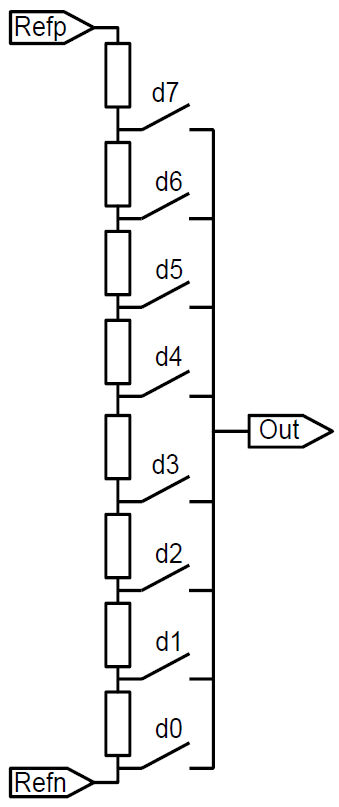
\includegraphics[height=3cm]{images/string_DAC.png}	% naja...
\end{minipage}
\hfill
\begin{minipage}[c]{0.8\columnwidth}
    Jeweils nur \textbf{ein Schalter} geschlossen

    \vspace{0.1cm}

    \begin{minipage}[c]{0.48\columnwidth}
        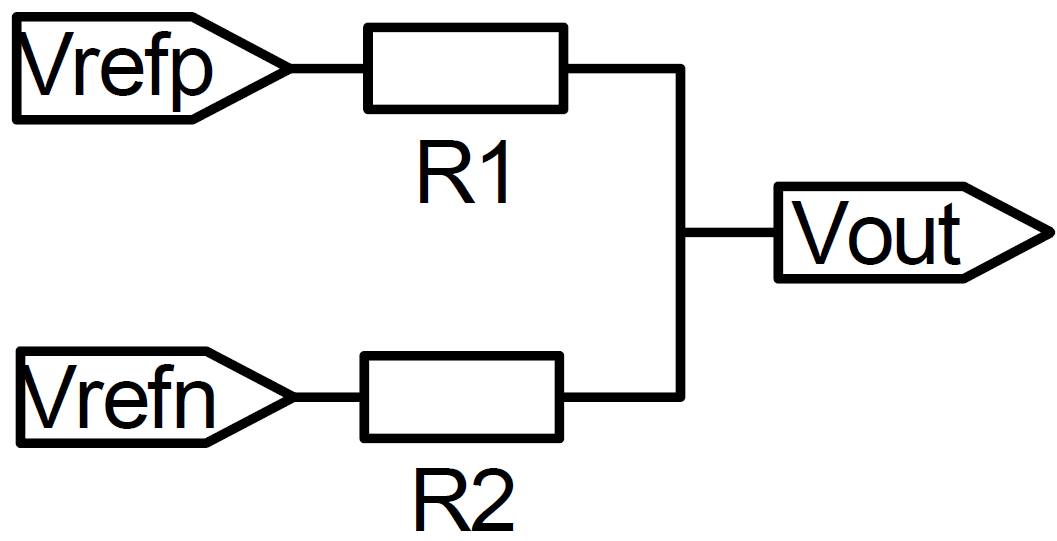
\includegraphics[width=0.95\columnwidth]{images/string_DAC_ersatzschaltung.png}
    \end{minipage}
    \hfill
    \begin{minipage}[c]{0.48\columnwidth}
        $R_1$: 1R \ldots 8R                                 \\
        $R_2$: 0R \ldots 7R                                 \\
        $V_{\rm out_{min}} = V_{\rm refn}$                  \\
        $V_{\rm out_{max}} = V_{\rm refp} - 1 \text{ LSB}$ 
    \end{minipage}

    \vspace{0.1cm}

    \begin{itemize}
        \item[+] Garantiert Stetigkeit
        \item \cbl{$2^n$ = Anzahl \textbf{Widerstände}} = Anzahl Schalter \textrightarrow\ $n$-to-$2^n$ Decoder
    \end{itemize}
\end{minipage}


\subsubsection{Voltage Scaling - String DAC (3 Bit)}

\begin{minipage}[c]{0.22\columnwidth}
    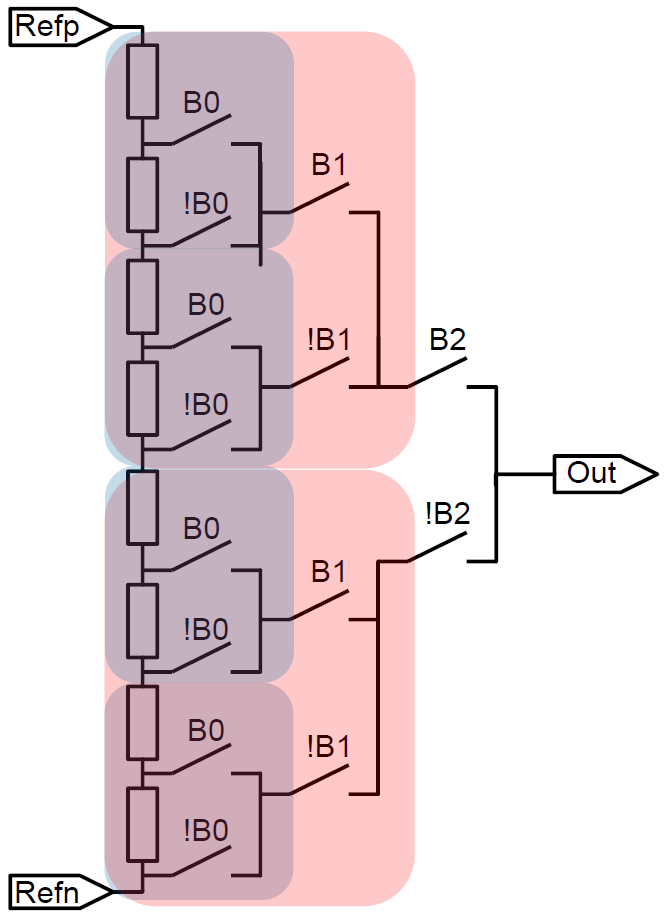
\includegraphics[width=\columnwidth]{images/string_DAC_advanced.png}
\end{minipage}
\hfill
\begin{minipage}[c]{0.76\columnwidth}
    Benötigt keinen Decoder aber zusätzliche Schalter

    \vspace{0.2cm}

    3-Bit DAC besteht aus: 

    \vspace{0.1cm}

    \begin{itemize}
        \item \cvt{4 mal 1-Bit DAC in Serie} 
        \item \crd{2 mal 2-Bit DAC in Serie}
    \end{itemize}

    \vspace{0.1cm}

    \textrightarrow\ Mit 2 mal 3-Bit DAC und Umschalter wird 4-Bit DAC gebaut
\end{minipage}


\subsubsection{Strom-DAC nach Parallelverfahren}

\begin{minipage}[c]{0.48\columnwidth}
    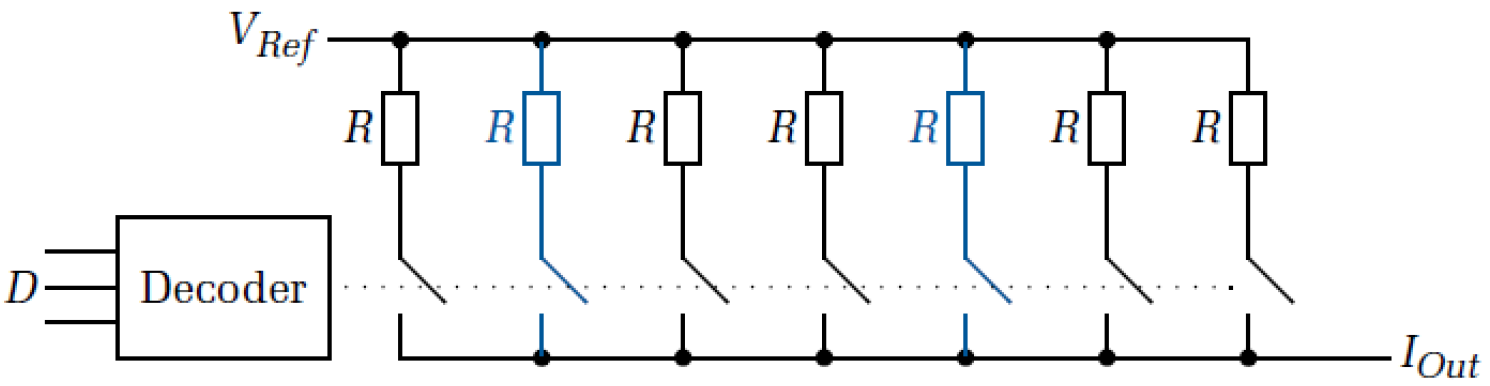
\includegraphics[width=\columnwidth]{images/strom_DAC_widerstaende.png} 
    $$ \boxed{ I_{\rm out} = D \frac{V_{\rm ref}}{R} } $$
\end{minipage}
\hfill
\begin{minipage}[c]{0.48\columnwidth}
    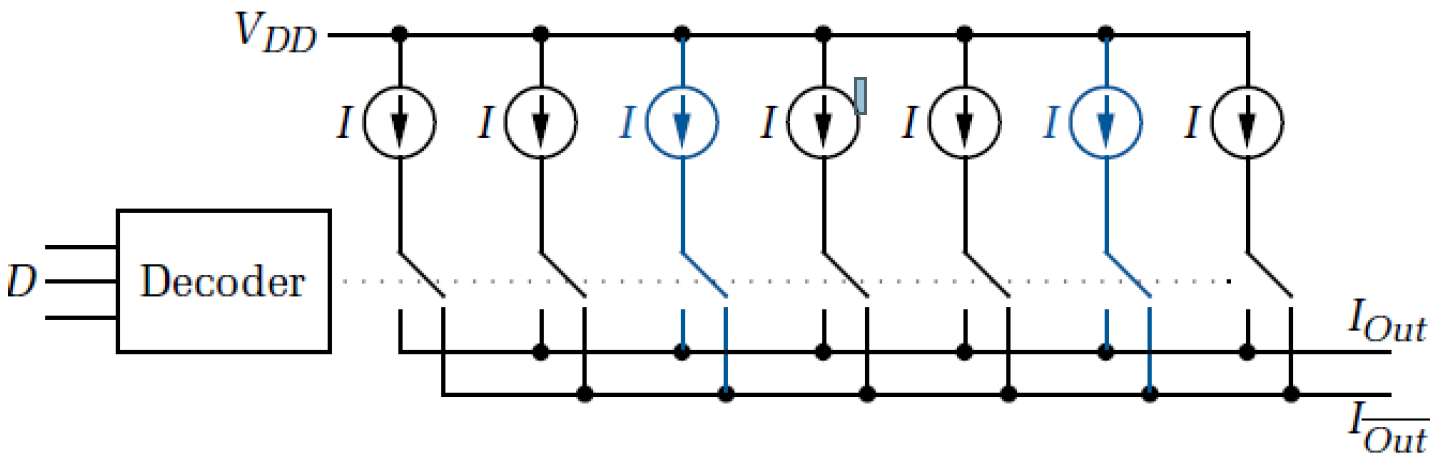
\includegraphics[width=\columnwidth]{images/strom_DAC_stromquellen.png}
    $$ \boxed{ I_{\rm out} = D \cdot I } $$
\end{minipage}

\vspace{0.2cm}

Um eine Ausgangsspannung $V_{\rm out}$ zu erhalten, wird ein OPV nachgeschaltet gemäss Kapitel \ref{R2R}


\subsection{Wägeverfahren}

\subsubsection{Wägeverfahren -- resistiv}

\begin{minipage}[c]{0.4\columnwidth}
    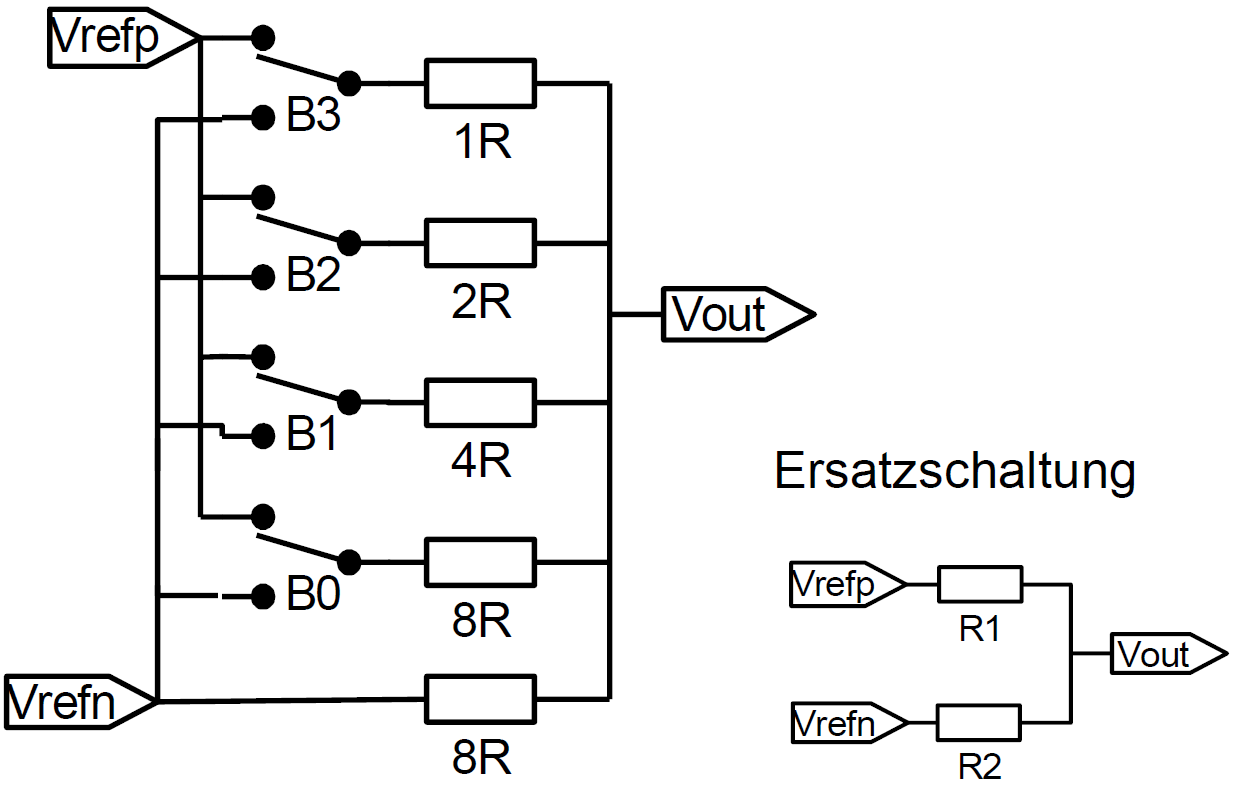
\includegraphics[width=\columnwidth]{images/waegeverfahren.png}
\end{minipage}
\hfill
\begin{minipage}[c]{0.56\columnwidth}
    \begin{itemize}
        \item[+] $N$ Widerstände, $n$ Schalter (Bits)
        \item[-] Nicht garantiert stetig
        \item[-] Grosser Wertebereich der Widerstände nötig 
    \end{itemize}

    $$ \textbf{Leitwerte!} \qquad \bm{G_0 = \frac{1}{8R} } $$
\end{minipage}

Bit $B_i$ schaltet Leitwert $2^i \cdot G_0$ nach $V_{\rm refp}$ (sonst $V_{\rm refn}$), Gesamtleitwert $2^n \cdot G_0$ \textrightarrow\ $G_0$ kürzt sich:
$$ \boxed{ V_{\rm out} = \frac{D}{2^n} (V_{\rm refp}- V_{\rm refn}) + V_{\rm refn} = D \cdot q + V_{\rm refn} } $$


\subsubsection{Kapazitiver DAC ohne Ausgangsbuffer (4 Bit)}

\begin{center}
    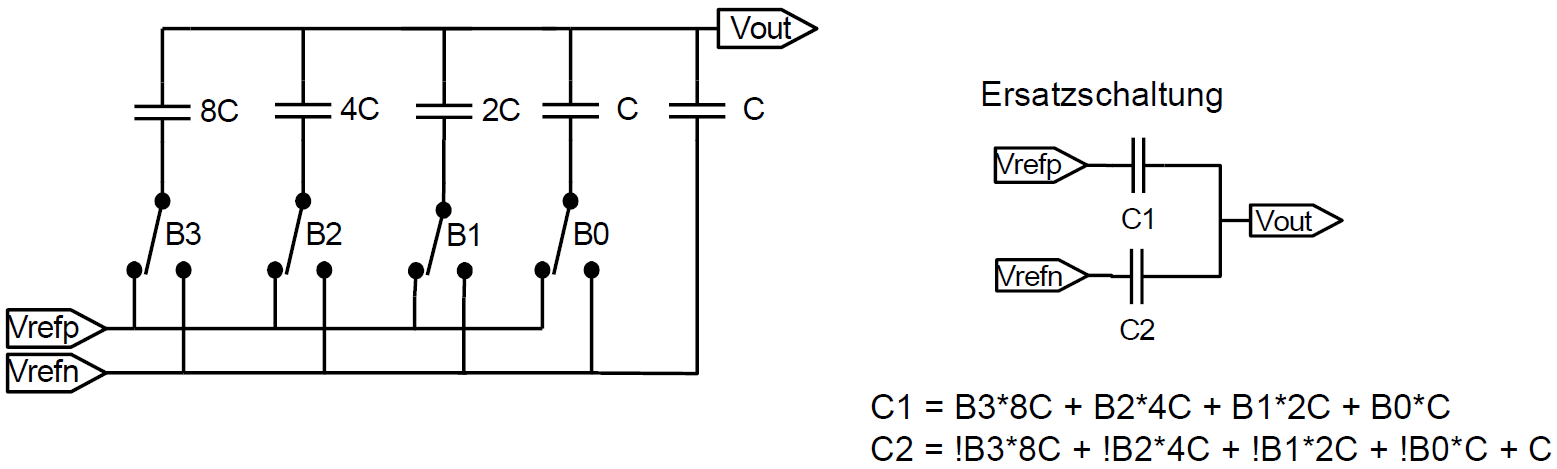
\includegraphics[width=0.85\columnwidth]{images/kapazitiver_DAC_2.png}
\end{center}

\textbf{Ladungserhaltung:} Ladung der Platten am Knoten $V_{\rm out}$ bleibt konstant, \mbox{$Q = C \cdot \Delta V$} \textrightarrow\ Teiler Kap.~\ref{cap-teiler} \\
Wenn Kapazitäten entladen sind, bevor geschaltet wird: 
$$ \boxed{ V_{\rm out} = \frac{C_1}{C_1 + C_2} (V_{\rm refp} - V_{\rm refn}) + V_{\rm refn}  \quad  \text{mit } C_1 + C_2 = 2^n \cdot C } $$

\textbf{Problem:} Lastkapazitäten an $V_{\rm out}$ \textrightarrow\ Schaltung so schlecht brauchbar  


\subsubsection{Kapazitiver DAC mit Ausgangsbuffer}

\begin{minipage}[c]{0.44\columnwidth}
    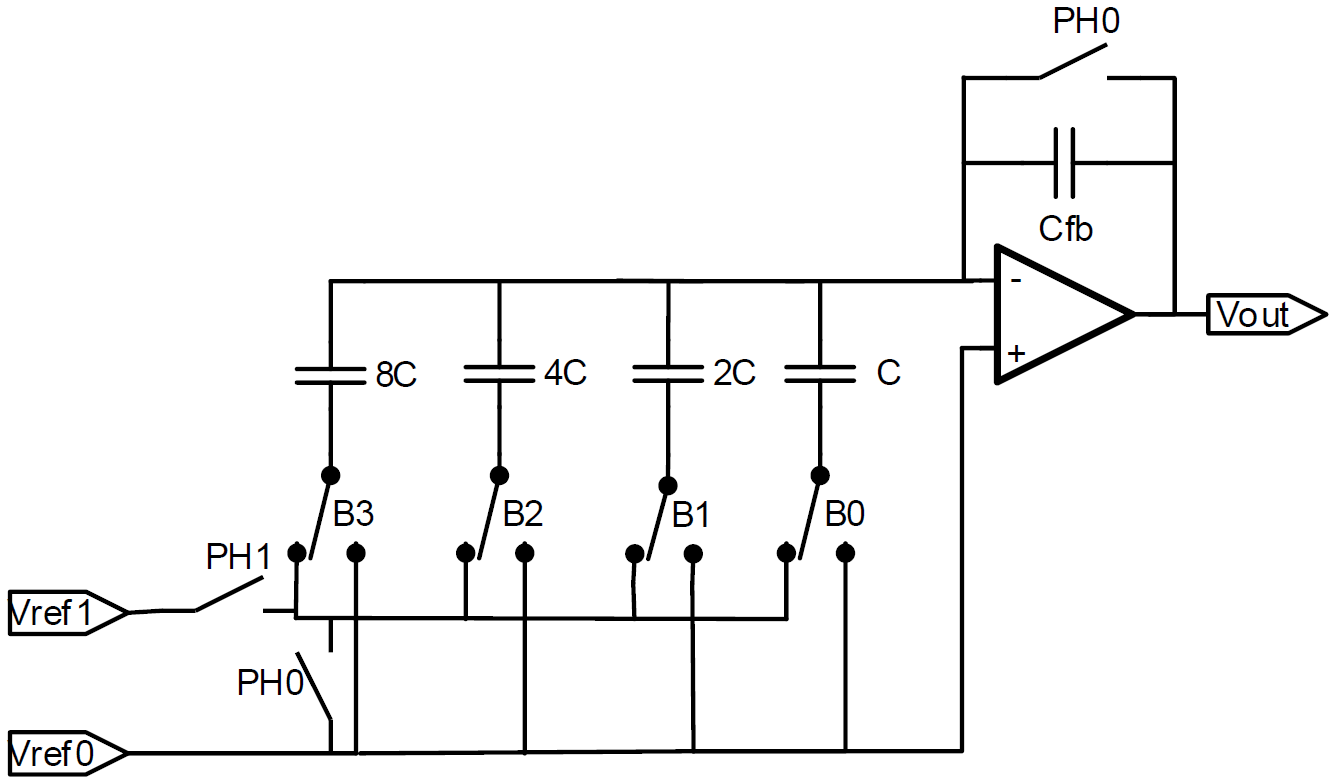
\includegraphics[width=\columnwidth]{images/kapazitiver_DAC_ausgangsbuffer.png}
\end{minipage}
\hfill
\begin{minipage}[c]{0.55\columnwidth}
    \raggedright
    \cbl{Bit $B_i = 1$: Kondensator an $V_{\rm ref1}$, sonst an $V_{\rm ref0}$} \\
    2 Phasen: PH0 und PH1

    PH0: $V_{\rm out} = V_{\rm ref0}$ (Ladungen resettate)\\
    PH1: Ausgang gültig (nach Einschwingen)

    $$ \boxed{ V_{\rm out} = -(V_{\rm ref1} - V_{\rm ref0}) \cdot \frac{\cbl{C_{\rm tot}}}{C_{fb}} + V_{\rm ref0} } $$
\end{minipage}\smallbreak

\cbl{$C_{\rm tot}$} = Summe der an $V_{\rm ref1}$ geschalteten Kondensatoren $= \sum_i B_i\, 2^i C$ \\ \textbf{Ladungserhaltung} am $-$-Knoten: Kap.~\ref{cap-teiler}

\vspace{0.2cm}

\textbf{Nachteil:} Sample-Hold nötig für Ausgangsspannung in Phase PH0 (wenn Schalterstellung gewechselt wird)


\subsubsection{Wägeverfahren mit Widerständen und Ausgangsverstärker}

\begin{minipage}[c]{0.45\columnwidth}
    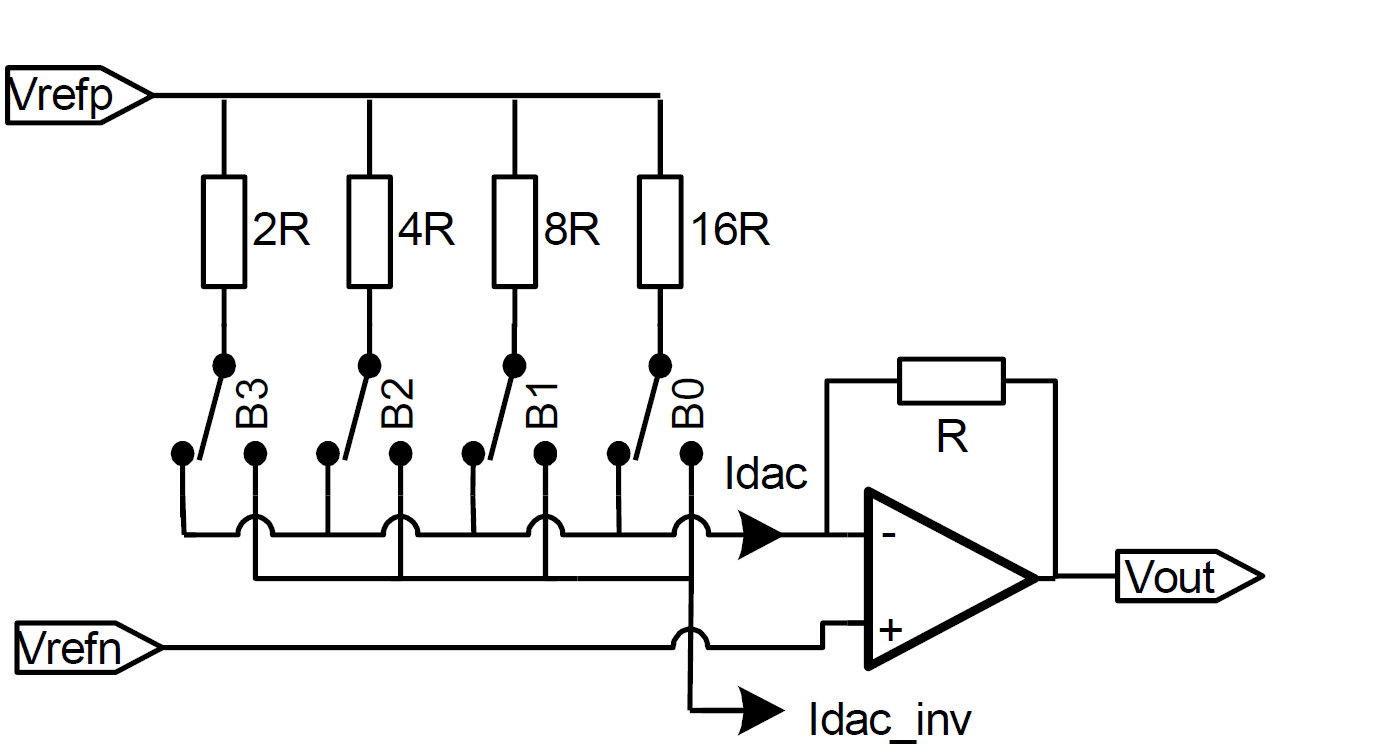
\includegraphics[width=\columnwidth]{images/DAC_ausgangsverstaerker.png}
\end{minipage}
\hfill
\begin{minipage}[c]{0.53\columnwidth}
    $$ \boxed{ I_{\rm dac_{max}} = \frac{V_{\rm refp} - V_{\rm refn}}{R_{\rm LSB}} (2^n -1) } $$
    $$ \boxed{ I_{\rm dac} = \frac{V_{\rm refp} - V_{\rm refn}}{R_{\rm LSB}} \, D } $$
    $$ \boxed{ V_{\rm out} = V_{\rm refn} - R_{fb} \cdot I_{\rm dac} } $$

    \vspace{0.2cm}
    \begin{itemize}
        \item[+] differentiell ($I_{\rm dac_{inv}}$)
        \item[-] Ausgang darf belastet werden
    \end{itemize}
\end{minipage}

\textbf{Binär gewichtet:} $R_i = R_{\rm LSB}/2^i$ (Bit $B_i$), $R_{\rm LSB}$ = \textbf{grösster} $R_i$ \textrightarrow\ $\boxed{ |q| = \frac{R_{fb}}{R_{\rm LSB}} \cdot |\Delta V_{\rm ref}| }$ \\

\subsubsection{DAC mit R2R-Netzwerk}
\label{R2R}

\begin{minipage}[c]{0.43\columnwidth}
    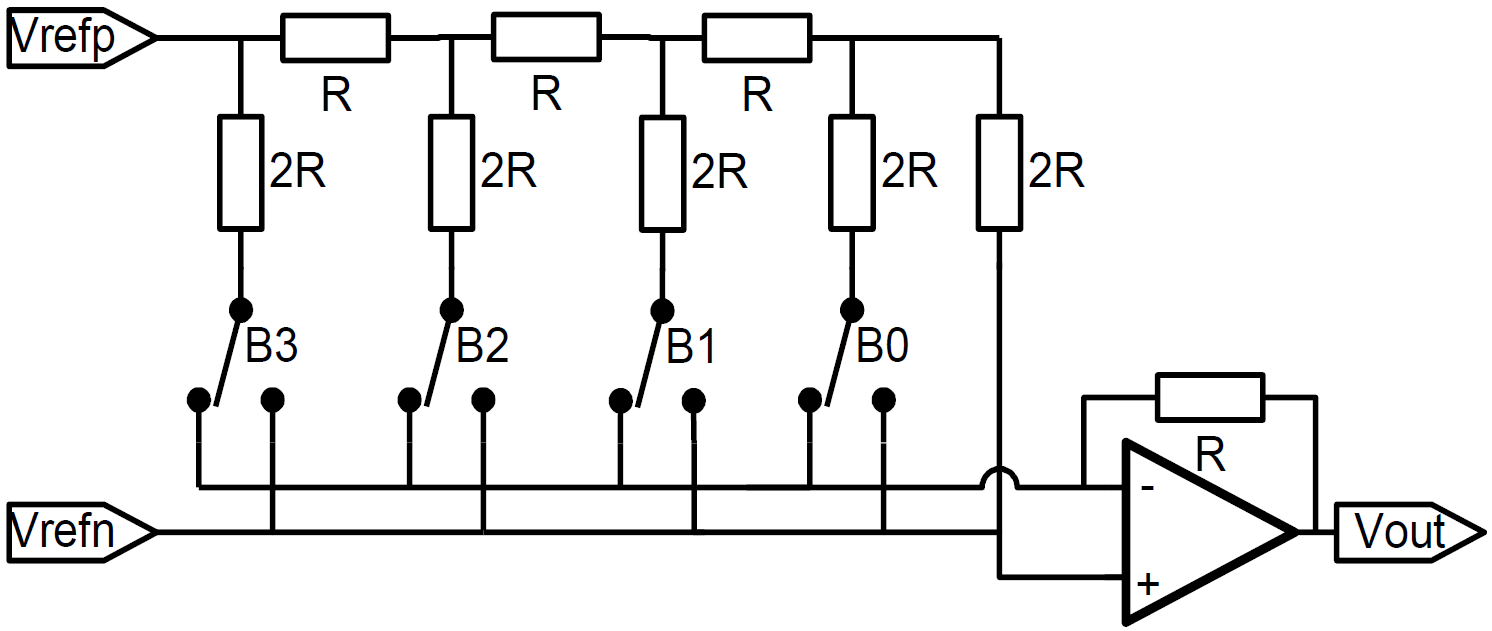
\includegraphics[width=\columnwidth]{images/R2R_netzwerk}
\end{minipage}
\hfill
\begin{minipage}[c]{0.56\columnwidth}
    Für Ersatzwiderstand \textbf{von rechts} her 'schauen'

    {(\footnotesize R si combinano sempre creando Part. U con
    \tikz[baseline=-0.5ex, line width=0.2pt]{
        \draw (0,0) -- (0.2,0) node[draw, minimum width=0.4cm, minimum height=0.2cm, inner sep=0pt, anchor=west] (a) {\tiny R} (a.east) -- ++(0.2,0)
        node[draw, minimum width=0.4cm, minimum height=0.2cm, inner sep=0pt, anchor=west] (b) {\tiny R} (b.east) -- ++(0.2,0);
    })}

    \vspace{0.2cm}
    
    \begin{itemize}
        \item[+] Nur 2 Widerstandswerte: R, 2R
        \item[+] Gute Alternative zu gewichteten R's bzw. C's
        \item[+] Stromgewichtung über Spannungsteiler von $V_{\rm refp}$ zu $V_{\rm refn}$
    \end{itemize}
\end{minipage}

\vspace{0.2cm}
Variiert $V_{\rm refp}$, dann variiert auch $V_{\rm out}$

\textbf{Jeder geschlossene Schalter trägt gewichtet zur Ausgangsspannung bei! \\
\crd{Achtung: Invertierung!}}

$$ \boxed{V_{\rm out} = V_{\rm refn} - (V_{\rm refp} - V_{\rm refn}) \cdot \frac{D}{2^n}}  $$\vspace{-0.5em}

{\footnotesize $n$ = Anzahl Bits, \quad $D = \sum_i B_i\, 2^i$ = 
Dezimalwert des Digitalworts (z.B.\ $1010_2 = 8 + 2 = 10$)\\
\textbf{Mit Buffer statt Opamp (nicht invertierend):} $V_{\rm out} = V_{\rm refn} + (V_{\rm refp} - V_{\rm refn}) \frac{D}{2^n}$ \\
Herleitung: Thévenin Knoten für Knoten, $R_{\rm th} = R$ konstant, $V_{\rm th}$ halbiert sich pro Knoten (Teiler \textbf{nicht} multiplizieren!)}\smallbreak


\cbl{\myul{\textbf{Beispiel:}}

\renewcommand{\arraystretch}{1.8}
\begin{tabular}{lll}
    $B_3 \text{ geschlossen: } V_{\rm out} = V_{\rm refn} - \frac{\Delta V_{\rm ref}}{2}$    & & 
    $B_2 \text{ geschlossen: } V_{\rm out} = V_{\rm refn} - \frac{\Delta V_{\rm ref}}{4}$    \\
    $B_1 \text{ geschlossen: } V_{\rm out} = V_{\rm refn} - \frac{\Delta V_{\rm ref}}{8}$    & & 
    $B_0 \text{ geschlossen: } V_{\rm out} = V_{\rm refn} - \frac{\Delta V_{\rm ref}}{16}$
\end{tabular}
}
\renewcommand{\arraystretch}{1}

\subsection{Zählverfahren (PWM)}

\subsubsection{PWM: Pulse Width Modulation}

\begin{minipage}[c]{0.45\columnwidth}
    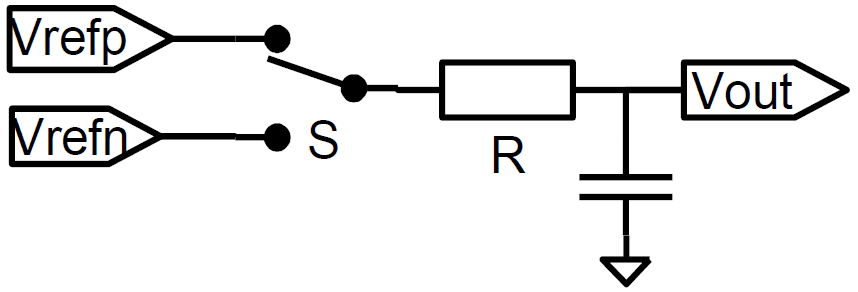
\includegraphics[width=\columnwidth]{images/PWM_DAC}
\end{minipage}
\hfill
\begin{minipage}[c]{0.52\columnwidth}
    \raggedright
    $S$ schaltet zwischen $V_{\rm refp}$ und $V_{\rm refn}$ (\textrightarrow\ PWM) \\
    (\textrightarrow\ meistens $V_{\rm ref}$ und $GND$ )

    \vspace{0.2cm}

    \textbf{RC glättet und erzeugt 'DC'}
\end{minipage}

\vspace{0.2cm}

\begin{minipage}[c]{0.48\columnwidth}
    \begin{itemize}
        \item[+] Sehr einfache Schaltung
        \item[+] Ermöglicht hohe Auflösung 
        \item[+] Funktioniert onchip digital (z.B. FPGA, $\mu$C) \textrightarrow\ analoge Schaltung extern
    \end{itemize}
\end{minipage}
\hfill
\begin{minipage}[c]{0.48\columnwidth}
    \raggedright
    \begin{itemize}
        \item[-] Sehr langsam
        \item[-] Benötigt grosses $\tau$ für kleine Spannungsrippel (oder Tiefpass höherer Ordnung)
    \end{itemize}
\end{minipage}



\myul{\textbf{PWM-Ansteuerung für Schalter $\bm{S}$}}

\begin{minipage}{0.4\columnwidth}
    \centering $$ \boxed{ \overline{V_{\rm out}} = V_{\rm refn} + (V_{\rm refp} - V_{\rm refn}) \cdot \frac{n}{N} }$$
\end{minipage}
\hfill
\begin{minipage}[c]{0.58\columnwidth}
    % LTeX: enabled=false
\resizebox{\columnwidth}{!}{
    \begin{tikzpicture}[yscale=0.55]
        \tikzstyle{every node}=[font=\LARGE]
        \useasboundingbox (-1.2,-3.0) rectangle (16,3.3);
        % V_ref (PWM)
        \draw[line width=2.5pt] (0,0) -- (0.000,0) -- (0.000,3.0) -- (2.100,3.0) -- (2.100,0) -- (3.500,0) -- (3.500,3.0) -- (5.600,3.0) -- (5.600,0) -- (7.000,0) -- (7.000,3.0) -- (9.100,3.0) -- (9.100,0) -- (10.500,0) -- (10.500,3.0) -- (12.600,3.0) -- (12.600,0) -- (14.500,0);
        % mittlere Spannung
        \draw[dashed, line width=1.5pt, red] (0,1.800) -- (14.500,1.800);
        % reale Ausgangsspannung (RC-Tiefpass)
        \draw[line width=3pt, blue] plot[smooth, tension=0.5] coordinates {(0.000,1.395) (0.087,1.439) (0.175,1.482) (0.262,1.524) (0.350,1.564) (0.438,1.603) (0.525,1.642) (0.612,1.679) (0.700,1.715) (0.787,1.750) (0.875,1.784) (0.962,1.818) (1.050,1.850) (1.137,1.882) (1.225,1.912) (1.312,1.942) (1.400,1.971) (1.487,1.999) (1.575,2.027) (1.662,2.053) (1.750,2.079) (1.837,2.105) (1.925,2.129) (2.012,2.153) (2.100,2.176) (2.188,2.116) (2.275,2.059) (2.362,2.002) (2.450,1.947) (2.537,1.894) (2.625,1.842) (2.712,1.792) (2.800,1.742) (2.887,1.695) (2.975,1.648) (3.062,1.603) (3.150,1.559) (3.237,1.517) (3.325,1.475) (3.412,1.435) (3.500,1.395) (3.587,1.439) (3.675,1.482) (3.762,1.524) (3.850,1.564) (3.937,1.603) (4.025,1.642) (4.112,1.679) (4.200,1.715) (4.287,1.750) (4.375,1.784) (4.462,1.818) (4.550,1.850) (4.637,1.882) (4.725,1.912) (4.812,1.942) (4.900,1.971) (4.987,1.999) (5.075,2.027) (5.162,2.053) (5.250,2.079) (5.337,2.105) (5.425,2.129) (5.512,2.153) (5.600,2.176) (5.688,2.116) (5.775,2.059) (5.862,2.002) (5.950,1.947) (6.037,1.894) (6.125,1.842) (6.212,1.792) (6.300,1.742) (6.387,1.695) (6.475,1.648) (6.562,1.603) (6.650,1.559) (6.737,1.517) (6.825,1.475) (6.912,1.435) (7.000,1.395) (7.087,1.439) (7.175,1.482) (7.262,1.524) (7.350,1.564) (7.437,1.603) (7.525,1.642) (7.612,1.679) (7.700,1.715) (7.787,1.750) (7.875,1.784) (7.962,1.818) (8.050,1.850) (8.137,1.882) (8.225,1.912) (8.312,1.942) (8.400,1.971) (8.487,1.999) (8.575,2.027) (8.662,2.053) (8.750,2.079) (8.837,2.105) (8.925,2.129) (9.012,2.153) (9.100,2.176) (9.188,2.116) (9.275,2.059) (9.362,2.002) (9.450,1.947) (9.537,1.894) (9.625,1.842) (9.712,1.792) (9.800,1.742) (9.887,1.695) (9.975,1.648) (10.062,1.603) (10.150,1.559) (10.237,1.517) (10.325,1.475) (10.412,1.435) (10.500,1.395) (10.587,1.439) (10.675,1.482) (10.762,1.524) (10.850,1.564) (10.938,1.603) (11.025,1.642) (11.112,1.679) (11.200,1.715) (11.287,1.750) (11.375,1.784) (11.462,1.818) (11.550,1.850) (11.637,1.882) (11.725,1.912) (11.812,1.942) (11.900,1.971) (11.987,1.999) (12.075,2.027) (12.162,2.053) (12.250,2.079) (12.337,2.105) (12.425,2.129) (12.512,2.153) (12.600,2.176) (12.688,2.116) (12.775,2.059) (12.862,2.002) (12.950,1.947) (13.037,1.894) (13.125,1.842) (13.212,1.792) (13.300,1.742) (13.387,1.695) (13.475,1.648) (13.562,1.603) (13.650,1.559) (13.737,1.517) (13.825,1.475) (13.912,1.435) (14.000,1.395)};
        \node[anchor=east] at (-0.15,3.0) {$V_{\rm ref}$};
        \node[anchor=east] at (-0.15,0) {$0$};
        \node[anchor=west, red] at (14.600,2.350) {$\overline{V_{\rm out}}$};
        \node[anchor=west, blue] at (14.600,1.250) {$V_{\rm out}$};
        % Zeitangaben (1. Periode)
        \draw[dotted] (0,0) -- (0,-2.9) (2.100,0) -- (2.100,-1.6) (3.500,0) -- (3.500,-2.9);
        \draw[<->, >=Stealth, line width=1.5pt] (0,-1.4) -- (2.100,-1.4) node[midway, fill=white, inner sep=1pt]{$nT$};
        \draw[<->, >=Stealth, line width=1.5pt] (0,-2.5) -- (3.500,-2.5) node[midway, fill=white, inner sep=1pt]{$NT$};
    \end{tikzpicture}
}

\end{minipage}


\subsection{Kaskadierte Wandler und Mischformen}

\subsubsection{Kaskadierte DACs}

\begin{minipage}[c]{0.6\columnwidth}
    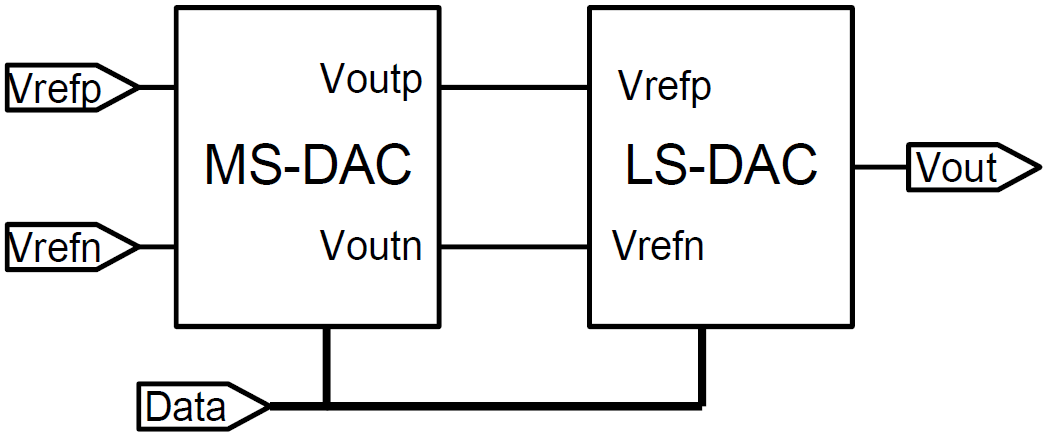
\includegraphics[width=0.75\columnwidth]{images/kaskadierte_DAC_1.png}
\end{minipage}
\hfill
\begin{minipage}[c]{0.38\columnwidth}
    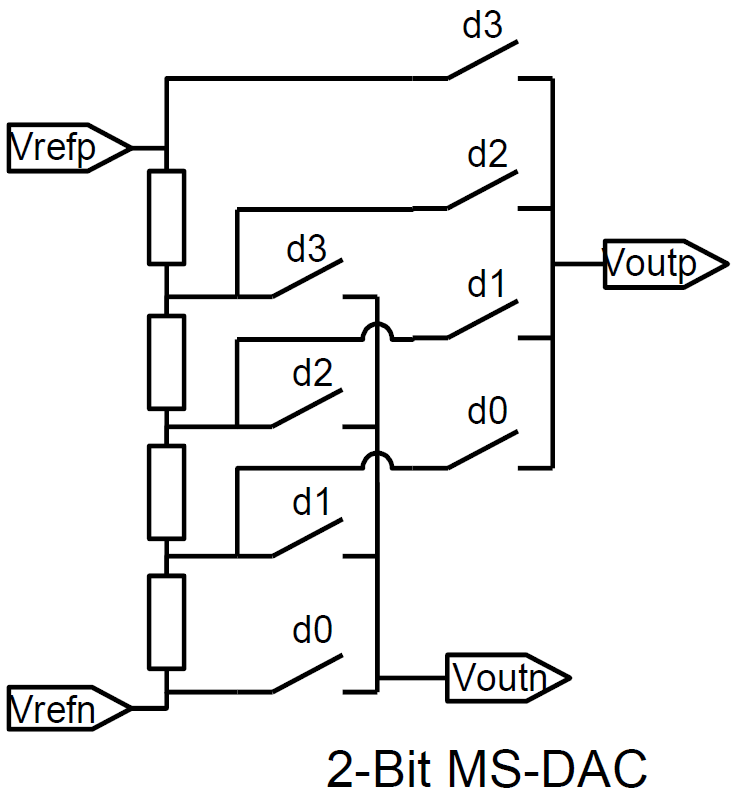
\includegraphics[width=0.7\columnwidth]{images/kaskadierte_DAC_2.png}
\end{minipage}

\vspace{0.2cm}

\begin{itemize}
    \item MS-DAC: 2 Ausgangsspannungen (über / unter gewünschtem $V_{\rm out}$)
    \item LS-DAC: folglich kleinere Eingangsspannungsdifferenz \\
        \textrightarrow\ Kleinerer Quantisierungsschritt $q$ \\
        \textrightarrow\ Höhere absolute Spannungsauflösung
\end{itemize}


\subsubsection{Segmentierter String DAC}

\begin{minipage}[c]{0.3\columnwidth}
    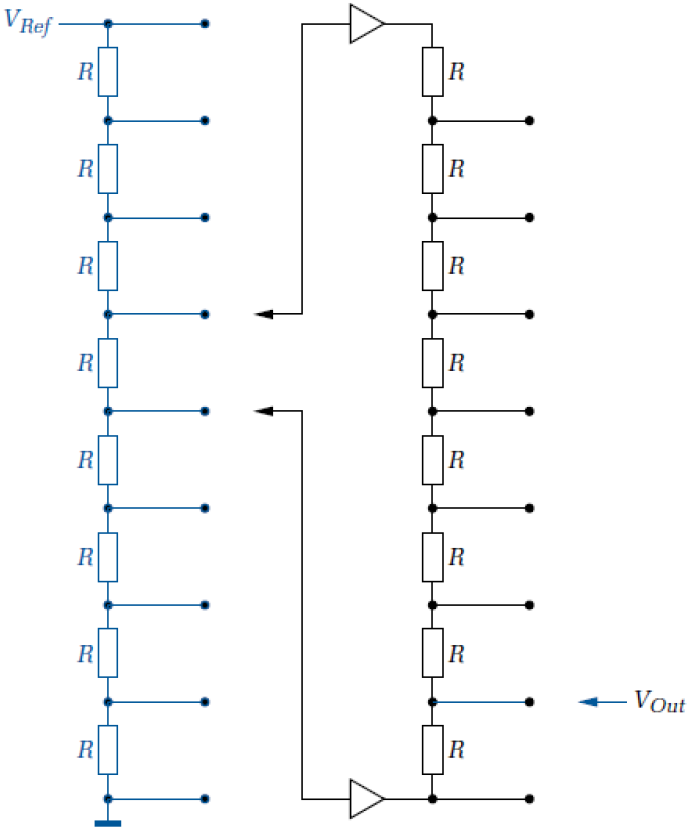
\includegraphics[width=\columnwidth]{images/segmented_string.png} 
\end{minipage}
\hfill
\begin{minipage}[c]{0.68\columnwidth}
    \begin{itemize}
        \item 2 'Strings' mit tiefer Auflösung ergeben doppelte\\
            Auflösung \textrightarrow\ $2 \cdot 8$R \textrightarrow\ $2 \cdot 3$ Bit
        
        \vspace{0.2cm}

        \item[+] Viel weniger Elemente
        \item[-] Benötigt 2 Buffer (damit keine Belastung des linkes 'Strings')
        \item[-] Buffer müsste offset-frei sein
    \end{itemize}

    \vspace{0.2cm}

    Alternative: Viel grössere R in rechtem 'String' \\
    \textrightarrow\ kleine Belastung links
\end{minipage}


\subsection{Zusammenfassung DACs}

    \begin{tabular}{ll}
    Parllelverfahren    & ... garantiert monotone Wandler           \\
    Wägeverfahren       & ... Anzahl Elemente nicht allzu hoch      \\
    Zählverfahren       & ... Wenn Zeit untergrodnete Rolle spielt
\end{tabular}

\vspace{0.2cm}

\textrightarrow\ \textbf{Oft werden Parallel- und Wägeverfahren kombiniert!}

\vspace{0.1cm}

Schnelle DACs haben oft einen Stromausgang und benötigen daher einen Ausgangsverstärker
\textrightarrow\ Ströme können schneller geschaltet werden als Spannungen!

\vspace{0.2cm}

Es gilt: Für optimale Resultate müssen \textbf{Kompromisse} eingegangen werden! 
